\documentclass[11pt,a4paper]{article}
\usepackage[spanish,es-nodecimaldot,es-noshorthands]{babel}
\usepackage[utf8]{inputenc}
\usepackage[margin=25mm]{geometry}
\usepackage{amsmath,amssymb,booktabs,tabularx,array,enumitem,hyperref,graphicx,caption,tikz,fancyhdr}
\usetikzlibrary{positioning}
\hypersetup{hidelinks,pdftitle={Documento explicativo del proyecto}}
\setlength{\parindent}{0pt}\setlength{\parskip}{6pt}\renewcommand{\arraystretch}{1.2}
\newcolumntype{Y}{>{\raggedright\arraybackslash}X}
\graphicspath{{figures/}}\captionsetup{font=small,labelfont=bf}
\pagestyle{fancy}\fancyhf{}\fancyhead[L]{\small Optimización de Cobertura Territorial mediante Grafos}\fancyhead[R]{\small Documento explicativo}\fancyfoot[C]{\thepage}
\begin{document}
\begin{titlepage}\centering\vspace*{38mm}
{\Large Universidad Diego Portales\par}\vspace{4mm}{\large Proyecto de Grafos y Algoritmos\par}\vspace{25mm}
{\LARGE\bfseries Optimización de Cobertura Territorial mediante Grafos\par}\vspace{8mm}
{\Large Documento explicativo de las simulaciones\par}\vfill
\begin{minipage}{.78\textwidth}\small\textbf{Propósito.} Explicar paso a paso cómo se construyen las simulaciones: desde los datos territoriales hasta la selección exacta de antenas y la lectura de sus mapas.\end{minipage}\vfill
{\large Octubre de 2026\par}\end{titlepage}

\section{Problema y recorrido de la simulación}
El proyecto desarrolla una simulación territorial para apoyar la planificación inicial de conectividad en zonas rurales. El punto de partida son localidades con población conocida y un conjunto de posibles ubicaciones para instalar antenas. Sin embargo, una ubicación cercana no siempre puede cubrir una localidad: el relieve puede interrumpir la línea de vista entre ambos puntos. Por esta razón, la simulación combina información geográfica, elevación del terreno y un modelo de grafos para distinguir las conexiones que sí son factibles bajo las reglas definidas.

Una vez construido ese conjunto de conexiones posibles, se busca decidir qué ubicaciones conviene seleccionar. El criterio es cubrir la mayor cantidad posible de población usando a lo más $k$ antenas. Si dos antenas alcanzan la misma localidad, su población se cuenta una sola vez; así, la decisión favorece combinaciones que complementan su cobertura territorial.

El proyecto se probó en dos ventanas piloto: una cercana a Yumbel, en la Región del Biobío, y otra en el sector rural de Paine/Buin, en la Región Metropolitana. Para cada una se generaron candidatos, se revisaron todos los segmentos candidato--localidad contra el relieve, se construyó el grafo de cobertura y se evaluaron todas las combinaciones admisibles mediante enumeración exacta. El resultado entrega las ubicaciones seleccionadas, la población cubierta, las aristas del grafo y mapas para interpretar espacialmente la decisión.

La pregunta que responde es:
\begin{quote}\itshape Si se pueden instalar hasta $k$ antenas, ¿en cuáles ubicaciones conviene instalarlas para cubrir la mayor cantidad posible de población?\end{quote}
La simulación sigue cinco pasos: (1) se delimita el territorio y se cargan los datos; (2) se generan candidatos; (3) se evalúan segmentos entre candidatos y localidades; (4) se construye el grafo y se resuelve por enumeración exacta; (5) se interpretan las métricas y mapas. El resultado es una evaluación de prefactibilidad: no certifica cobertura comercial ni autoriza la construcción de infraestructura.

\section{Paso 1: territorio y datos de entrada}
Se ejecutaron dos pilotos: una ventana cercana a Yumbel, Región del Biobío, y un sector rural de Paine/Buin, Región Metropolitana. Cada simulación parte de localidades con población, un área de estudio y un modelo digital de elevación (DEM). La Figura~\ref{fig:territorio} muestra las ventanas y su relieve.
\begin{figure}[h]\centering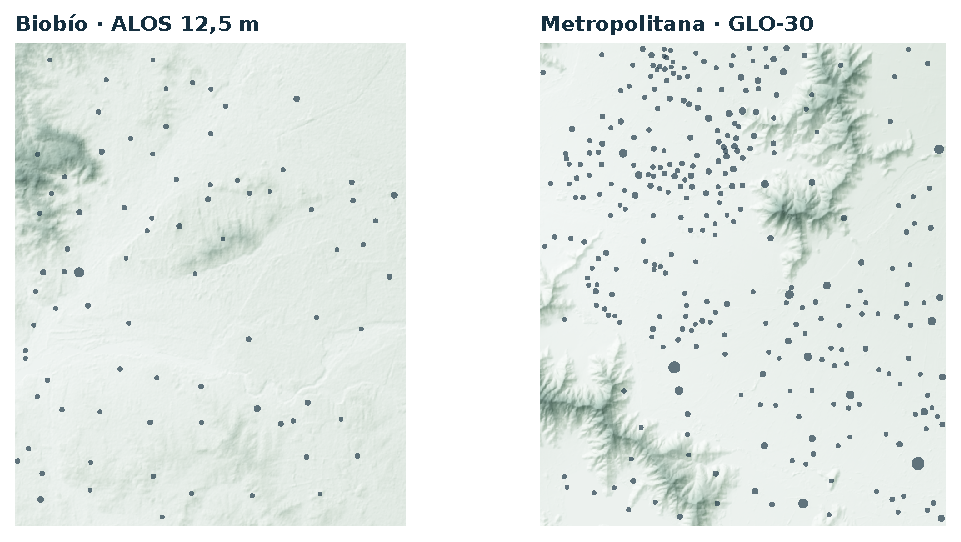
\includegraphics[width=.90\linewidth]{overview.pdf}\caption{Relieve y localidades incluidas: ventana cercana a Yumbel, Biobío (izquierda), y sector rural de Paine/Buin, Metropolitana (derecha).}\label{fig:territorio}\end{figure}

\subsection{Datos utilizados y previstos}
\begin{tabularx}{\linewidth}{@{}p{34mm}Yp{43mm}@{}}\toprule
\textbf{Dato}&\textbf{Uso en la simulación}&\textbf{Estado}\\\midrule
Localidades y población&Define los lugares que se desea cubrir y su peso poblacional.&V1 usa localidades SUBDERE basadas en Censo 2017.\\
Censo 2024 del INE&Debe aportar población y cartografía actualizada.&Previsto; aún no reemplaza la fuente del código actual.\\
Modelo digital de elevación&Permite revisar si el relieve bloquea cada enlace.&ALOS PALSAR en Biobío y Copernicus GLO-30 en Metropolitana.\\
Área de estudio&Delimita el territorio procesado.&Ventana geográfica o polígono.\\
Plan Regulador Comunal&Debe excluir ubicaciones incompatibles.&Previsto; aún no se aplica automáticamente en V1.\\\bottomrule\end{tabularx}

\subsection{Características de las ventanas piloto}
\begin{center}\small\begin{tabular}{@{}lrr@{}}\toprule
\textbf{Indicador}&\textbf{Biobío}&\textbf{Metropolitana}\\\midrule
Ubicación&Cercanías de Yumbel&Sector rural Paine/Buin\\
Ventana de estudio&18,39 $\times$ 22,71 km&19,05 $\times$ 22,65 km\\
Superficie procesada&417,63 km$^2$&431,48 km$^2$\\
DEM y resolución&ALOS, 12,5 m&Copernicus, 30 m\\
Elevación mínima--máxima&57--355 m&281--1.029 m\\
Localidades / candidatos&82 / 20&310 / 19\\
Segmentos evaluados&1.640&5.890\\
Con línea de vista&224 (13,66\%)&1.639 (27,83\%)\\
Bloqueados por relieve&1.416 (86,34\%)&4.251 (72,17\%)\\
Longitud mínima--máxima&0,53--25,60 km&0,03--25,92 km\\\bottomrule\end{tabular}\end{center}
Biobío presenta relieve bajo y ondulado; aun así, sus lomas intermedias bloquean muchos segmentos. Metropolitana presenta un relieve más contrastado. Estas cifras describen solamente las ventanas piloto y la grilla usada.

\section{Paso 2: candidatos, segmentos y grafo}
Se genera una grilla regular de candidatos dentro del área de estudio y se eliminan los puntos fuera del polígono o sobre celdas del DEM sin elevación válida. Para cada candidato y localidad se evalúa un segmento. El emisor se sitúa a 30 m sobre el terreno y el receptor a 1,5 m. Todos los segmentos están bajo el radio máximo de 30 km; un segmento sin arista fue descartado por obstrucción del relieve. El perfil se muestrea cada 6,25 m o menos en Biobío y cada 15 m o menos en Metropolitana. Sólo se crea una arista si ninguna muestra intermedia supera la recta de visión.

La información queda representada por un grafo bipartito $G=(A\cup D,E)$: $A$ es el conjunto de candidatos, $D$ el de localidades y $E$ los enlaces válidos. En la versión final el filtro PRC se aplicará antes de construir el grafo.
\begin{center}\begin{tikzpicture}[x=1cm,y=1cm]
\node[draw,circle,minimum size=8mm] (a1) at (0,1) {$a_1$};\node[draw,circle,minimum size=8mm] (a2) at (0,-1) {$a_2$};
\node[draw,circle,minimum size=8mm] (d1) at (5,1) {$d_1$};\node[draw,circle,minimum size=8mm] (d2) at (5,-1) {$d_2$};
\draw(a1)--(d1);\draw(a1)--(d2);\draw(a2)--(d2);\node[above=4mm of a1,font=\small\bfseries]{Candidatos};\node[above=4mm of d1,font=\small\bfseries]{Localidades};
\end{tikzpicture}\end{center}

\clearpage\subsection{Mapa de todos los segmentos evaluados}
La Figura~\ref{fig:segmentos} muestra la construcción del grafo antes de resolverlo. Cada recta une un candidato con una localidad. Las líneas verdes son los 224 segmentos de Biobío que superaron la línea de vista y forman las aristas del grafo; las naranjas son los 1.416 descartados por el relieve. Las estrellas corresponden a las cinco ubicaciones que seleccionará la solución exacta.
\begin{figure}[h]\centering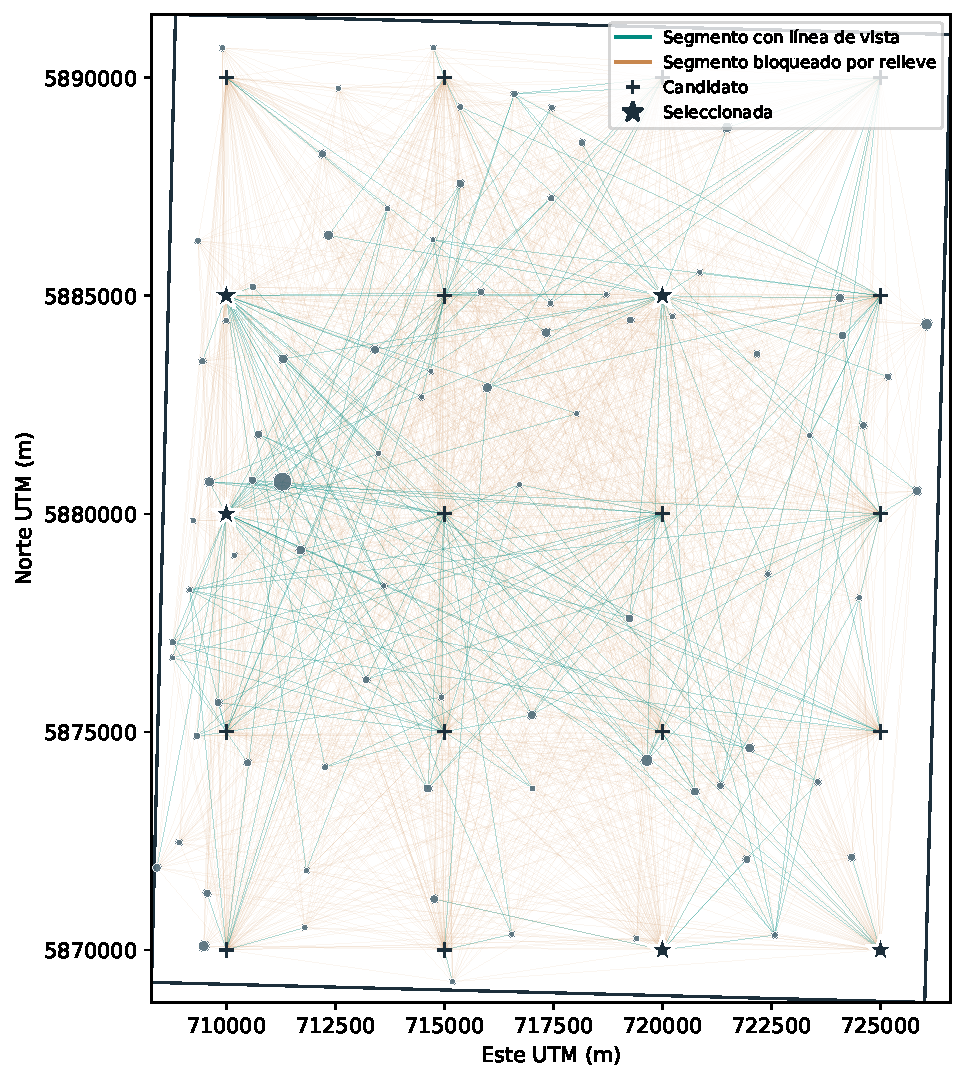
\includegraphics[width=.92\linewidth]{segmentos_biobio.pdf}\caption{Segmentos evaluados en la ventana cercana a Yumbel, Región del Biobío. Las líneas con visibilidad forman el conjunto de aristas del grafo bipartito.}\label{fig:segmentos}\end{figure}

\clearpage\subsection{Cómo se observa el grafo}
La Figura~\ref{fig:los} presenta un enlace visible y otro bloqueado. La Figura~\ref{fig:matriz} expresa el mismo grafo de Biobío como matriz: cada marca equivale a una arista entre un candidato y una localidad.
\begin{figure}[h]\centering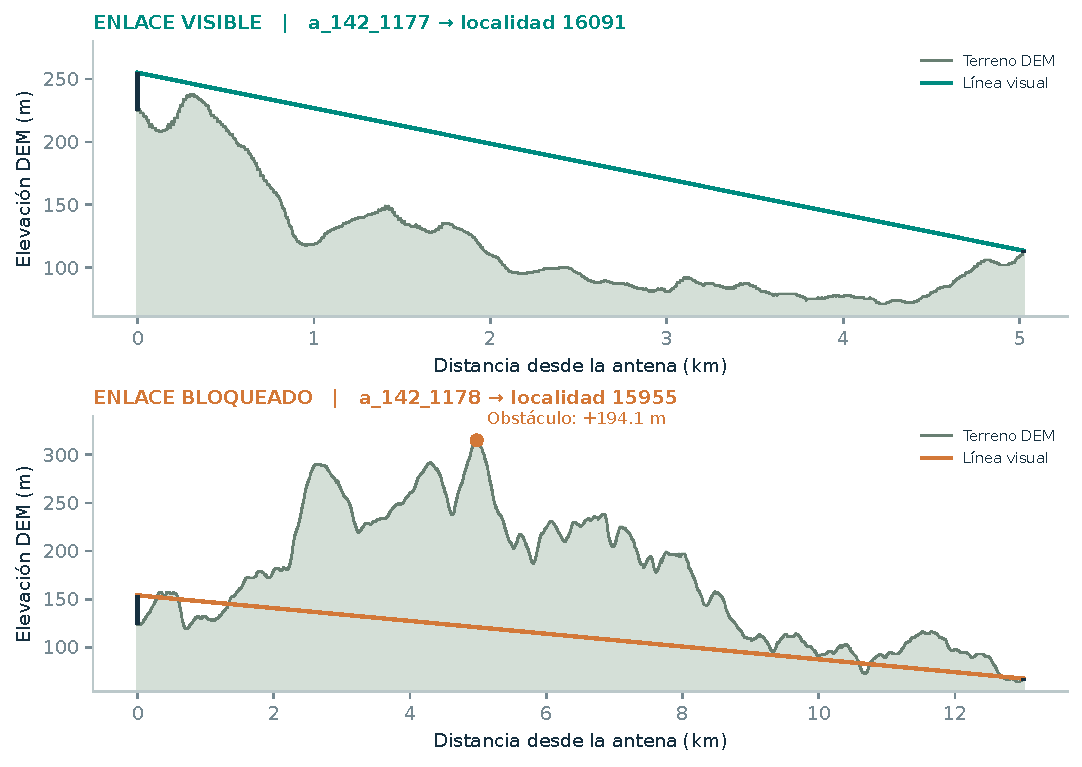
\includegraphics[width=.88\linewidth]{los_profiles.pdf}\caption{Ejemplos reales de un enlace visible y un enlace bloqueado en Biobío.}\label{fig:los}\end{figure}
\begin{figure}[h]\centering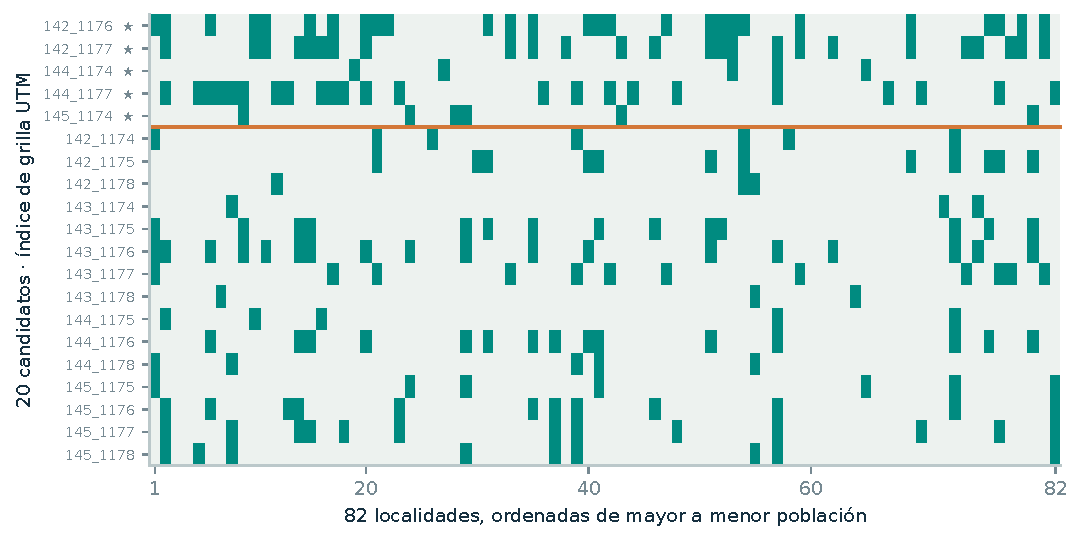
\includegraphics[width=\linewidth]{matrix.pdf}\caption{Matriz de adyacencia del grafo bipartito de Biobío.}\label{fig:matriz}\end{figure}

\clearpage\section{Paso 3: selección exacta de antenas}
Una localidad puede ser alcanzada por varias antenas, pero su población se cuenta una sola vez. Por eso se maximiza población única cubierta, no cantidad de enlaces. Sea $C(a)\subseteq D$ el conjunto de localidades cubiertas por $a$, $w_j$ la población de $d_j$ y $S$ el conjunto de antenas seleccionadas:
\[S\subseteq A,\qquad |S|\leq k.\]
\[\max_{S\subseteq A,\;|S|\leq k}\ \sum_{d_j\in\bigcup_{a\in S}C(a)}w_j.\]
La unión evita duplicar la población de una localidad. La formulación corresponde a \emph{Maximum Coverage} ponderado.

La solución usada es enumeración exacta: se generan todas las combinaciones admisibles de hasta $k$ candidatos, se calcula la población única cubierta y se conserva la mejor. Por ejemplo, con cuatro candidatos y dos antenas se revisan las seis parejas posibles. Como no se omite ninguna combinación, el resultado es óptimo para la instancia. Dado que las combinaciones crecen rápidamente, se usan áreas piloto acotadas y un límite de combinaciones.

\section{Paso 4: resultados de la solución exacta}
En ambas instancias se permite seleccionar hasta cinco antenas. La Figura~\ref{fig:comparacion} y la tabla resumen la solución óptima encontrada.
\begin{figure}[h]\centering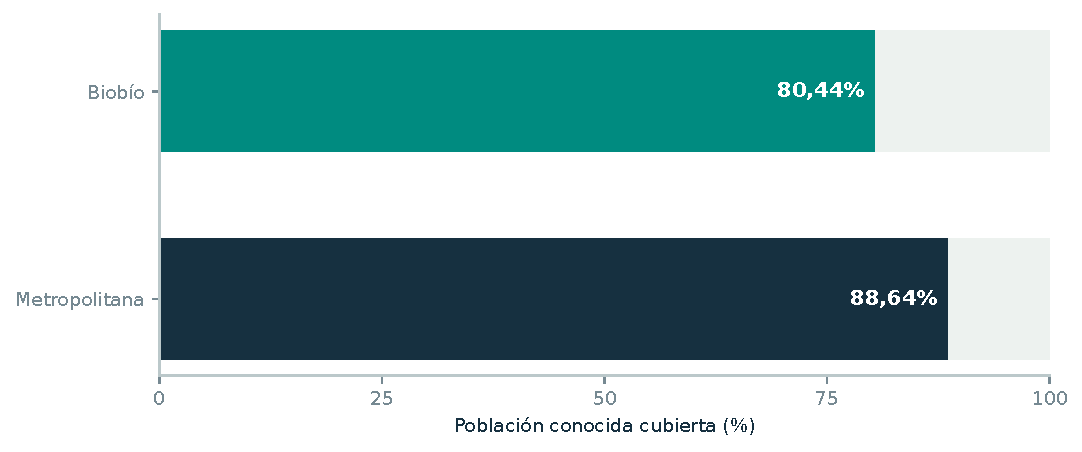
\includegraphics[width=.88\linewidth]{comparison.pdf}\caption{Porcentaje de población cubierta por la solución exacta.}\label{fig:comparacion}\end{figure}
\begin{center}\begin{tabular}{@{}lrrrr@{}}\toprule
\textbf{Piloto}&\textbf{Localidades}&\textbf{Candidatos}&\textbf{Población cubierta}&\textbf{Cobertura}\\\midrule
Biobío&82&20&4.210&80,44\%\\Metropolitana&310&19&25.119&88,64\%\\\bottomrule\end{tabular}\end{center}
En Biobío se construyeron 224 aristas y se evaluaron $\binom{20}{5}=15.504$ combinaciones. La solución óptima cubre 4.210 de 5.234 habitantes. En Metropolitana se construyeron 1.639 aristas y se evaluaron $\binom{19}{5}=11.628$ combinaciones; se cubren 25.119 de 28.337 habitantes. La cobertura superior de Metropolitana se explica por un grafo de cobertura más denso en esa ventana piloto.
\clearpage
Las primeras cinco filas de la matriz de Biobío corresponden a candidatos de la solución óptima. El gráfico muestra la población nueva aportada por cada uno, sin contar dos veces localidades compartidas.
\begin{figure}[h]\centering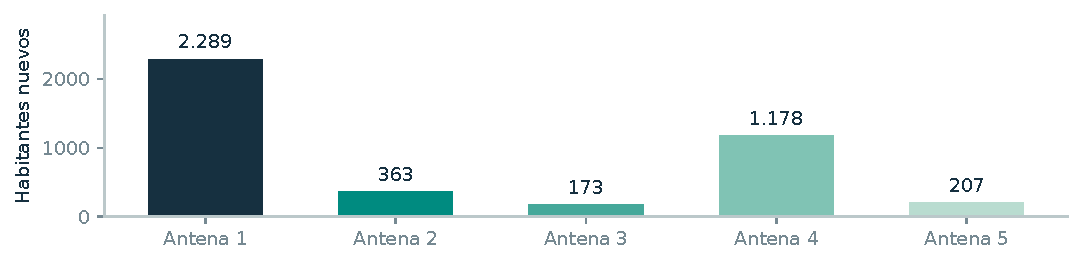
\includegraphics[width=\linewidth]{contributions.pdf}\caption{Contribuciones de población única de los cinco candidatos de la solución exacta de Biobío.}\end{figure}

\section{Paso 5: interpretación espacial y archivos generados}
Las estrellas representan las ubicaciones seleccionadas; los puntos verdes son localidades cubiertas y los naranjas no cubiertas bajo las reglas del modelo. Estos mapas permiten interpretar el resultado, pero no representan infraestructura instalada.
\begin{figure}[h]\centering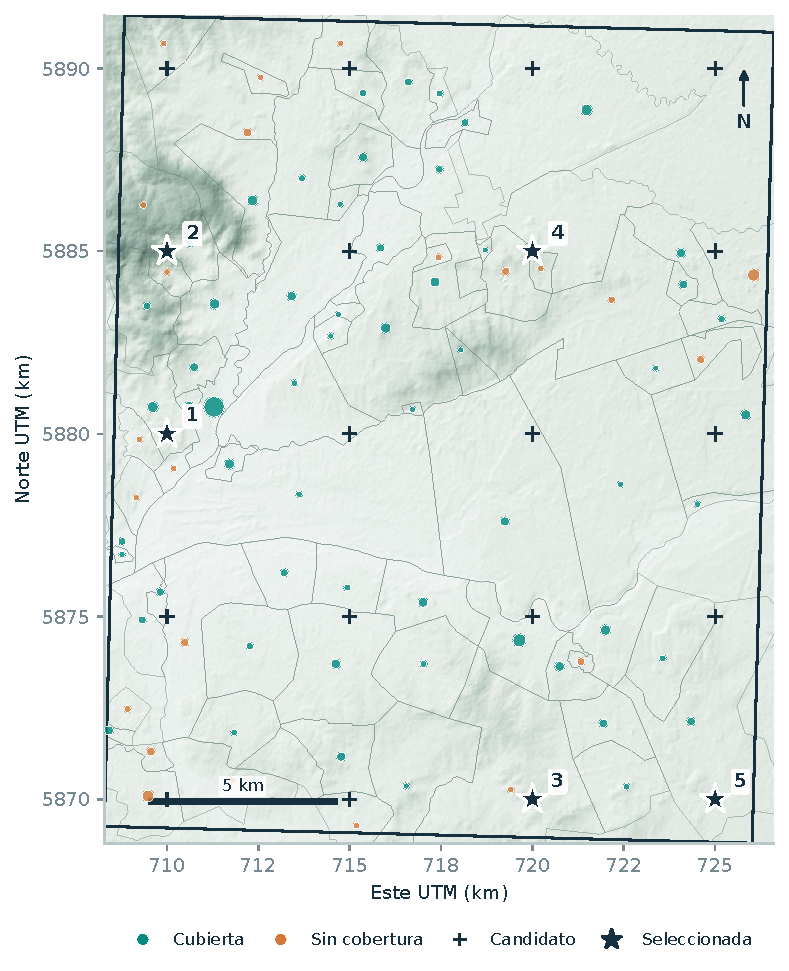
\includegraphics[width=.83\linewidth,height=.62\textheight,keepaspectratio]{map_biobio.pdf}\caption{Solución exacta para una ventana cercana a Yumbel, Región del Biobío ($72,65^\circ$ O a $72,45^\circ$ O; $37,30^\circ$ S a $37,10^\circ$ S), con $k=5$.}\end{figure}
\begin{figure}[h]\centering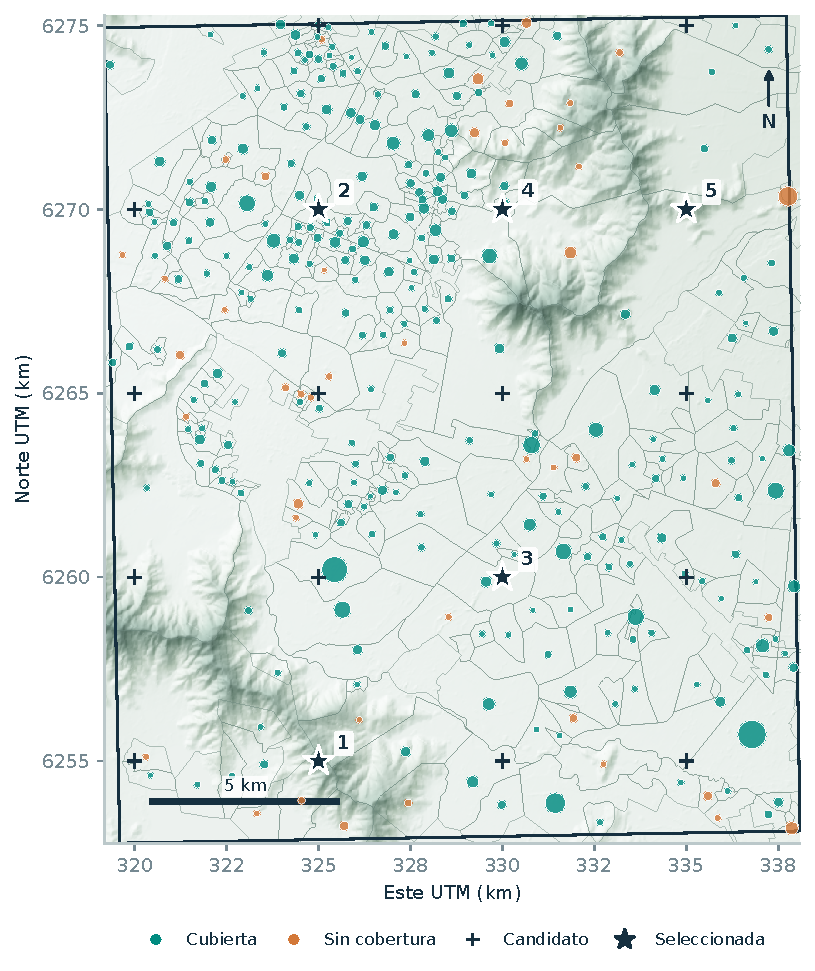
\includegraphics[width=.83\linewidth,height=.62\textheight,keepaspectratio]{map_metropolitana.pdf}\caption{Solución exacta para un sector rural de Paine/Buin, Región Metropolitana ($70,95^\circ$ O a $70,75^\circ$ O; $33,85^\circ$ S a $33,65^\circ$ S), con $k=5$.}\end{figure}
\clearpage
Cada ejecución produce el grafo de cobertura, antenas elegidas, población y porcentaje cubiertos, tiempo de ejecución, mapas, capas geográficas y un manifiesto con parámetros y fuentes. El mapa se genera reproyectando los datos a UTM, creando la grilla, evaluando pares candidato-localidad y destacando la solución exacta. También se exportan \texttt{demand.geojson}, \texttt{demand\_points.geojson}, \texttt{candidates.geojson} y \texttt{study\_area.geojson} para revisión en SIG.

El DEM permite una revisión geométrica del relieve. El modelo no incorpora propiedad del suelo, energía, acceso vial, permisos, vegetación, edificios, capacidad de red ni calidad de servicio. Por tanto, la selección es una recomendación de prefactibilidad y no demuestra que una torre pueda construirse en la práctica.

{\footnotesize \textbf{Fuentes de referencia.} Instituto Nacional de Estadísticas (INE), Censo de Población y Vivienda 2024 (\url{https://www.ine.gob.cl/}); SUBDERE, estudio de localidades basado en Censo 2017; ALOS PALSAR / CIREN-IDE Chile; Copernicus DEM GLO-30.\par}
\end{document}
